\chapter{Background}
\section{Observations In Space}
Observations of objects in space can be conducted both from Earth and from orbits in space.
\citet{Mons} talks about how performing astronomy from Earth is limited by the filtering and distortion of electromagnetic radiation by the Earth's atmosphere, a feature that protects life on Earth from ultraviolet rays, x-rays and gamma rays. The altitude needed to detect the different bands of the electromagnetic spectrum is illustrated in Fig. \ref{fig: em_surface}. From Earth radio waves, near-infrared and visible light are observable. For observing other frequencies of the electromagnetic spectrum it is necessary to have observatories in space where the atmosphere is not present. There are several ways of observing and examining objects in space. To make observations from space most often the equipment needed is launched  into space on board a satellite and the two most commonly used methods for examining astronomy objects in space are via \emph{Photometry} and \emph{Spectroscopy.}

\afterpage{
\begin{figure}[h]
\centering
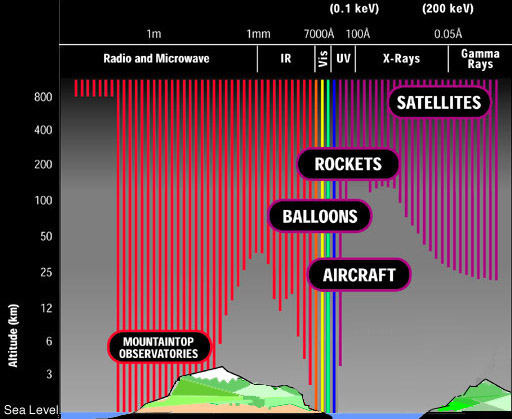
\includegraphics[width=.6\textwidth]{em_earth}
\caption[hej]{Illustration of the altitude needed to observe the different bands of the electromagnetic spectrum. Fig. from (Online).\footnotemark}
\label{fig: em_surface}
\end{figure}
\footnotetext{\url{http://migall.fastmail.fm.user.fm/astronomy/telescopes_detectors/emr/page6.htm}}
}

\section{The Space Mission Life Cycle and Architecture}
When planning a mission in space, a great amount of planning must first be done back on Earth. This is the case whether planning a manned mission or launching a satellite into orbit.
\citet{smad} gives a nice overview of the progress of designing a space mission:

\begin{itemize}
\item \emph{Concept exploration}, The initial study phase, in which a broad definition of the space mission and its components.

\item \emph{Detailed development}, the formal design phase, which results in a detailed definition of the system components and test of hardware and development.

\item \emph{Production and deployment}, the construction of the ground and flight hardware and launch of the final system. 

\item \emph{Operations and support}, the day-to-day operations of the space system, its maintenance and support, and its deorbit or recovery at the end of the mission life. 
\end{itemize}

Furthermore all space missions consist of a set of elements and the arrangement of these elements form the space mission architecture \citep{smad}.

The \textit{subject} of the mission is the object to be examined that either interacts with or is measured by the \textit{payload}.
\\

The \textit{payload} consist of the hardware and software that measure or interact with the subject. The payload is contained within the \textit{platform} which also holds all the subsystems that handle, altitude, orbit, power, telemetry and data. The \textit{payload} and \textit{platform} are together called the \textit{spacecraft}. The \textit{spacecraft} for the AU-SAT mission would be the satellite with a telescope, an onboard computer, for communications and onboard data processing and likely a spectrograph to analyze the incoming light from the stars. 
\\

The \textit{launch system} includes the launch facility and the launch vehicle that is needed to launch the payload into orbit. 
\\

The \textit{orbit} is the path or trajectory of the spacecraft. There are several orbits the spacecraft enters before it reaches its mission orbit. An often used orbit is the \textit{low earth orbit} with an altitude between 200-2000 \si{\kilo\meter}. Most satellites in orbit use the \textit{low earth orbit}, which is also used by the \textit{International Space Station} which houses the astronauts in space. 
\\

The \emph{ground systems} consist of the ground stations that connect with the spacecraft, so the operators are able to control the spacecraft and receive the 	telemetry and the mission data. 
\\

For the AU-SAT the Institute of Physics and Astronomy Aarhus University will decide the subject of the mission and determine the payload for the satellite. The scope of this bachelor's thesis is to examine the stability of the spectrograph that could be included in the payload if the satellite is launched. The spacecraft bus will be delivered by the Danish Cubesat company GomSpace. For the launch system, it will be required to buy a free spot on a commercial rocket, that would deliver the spacecraft on a desired orbit for observations. 

\section{Nanosatellites - Cubesats}
\label{satellite}
In the last decade launching a satellite into space has become more accessible with the introduction of smaller and cheaper nanosatellites, also called Cubesats. A Cubesat is small satellite made up of multiples of \num{10 x 10 x 10} \si{\centi\meter} cubic units. Cubesats are often build with off the shelf components for their electronics	 and structure. Only in recent time the technology has evolved to allow for high performance miniature star trackers, that are used to determine the orientation of the satellite in space. With a star tracker and a pointing controller, consisting of three axis reaction wheels used to rotate the satellite, the satellite is able to keep its needed orientation for observations in space \citep{brite}. As a satellite orbits around Earth it needs to rotate in order to keep pointing at the object being observed if observations are made over a long period of time. The continuous movement from the pointing of the satellite results in a change of how the light hits the light entrance of the satellite. Shown in Fig. \ref{fig: pointing} is a simulation for the BRITE telescope, of how a star being observed moves over the light entrance as a result of the pointing of the satellite. 
Satellites in orbit are also subject to temperature variations due to the satellite being exposed to direct sunlight or being in the shadow of the Earth. If build the AU-SAT will consist of six cubic units and will be tested to verify if can hold up to the environment in space.

\begin{figure}[h]
\centering
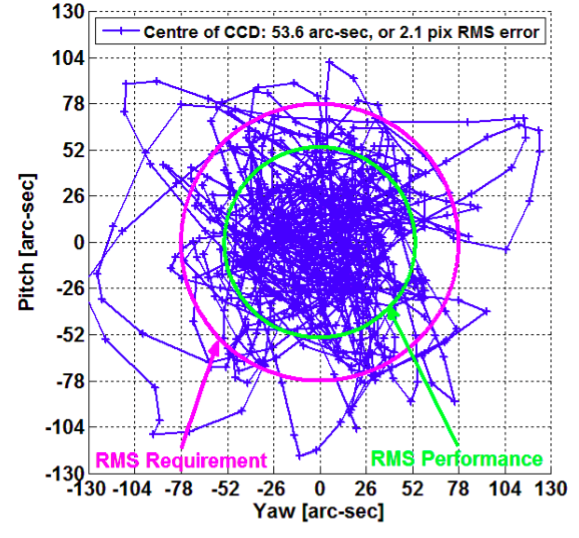
\includegraphics[width=.5\linewidth]{pointing.png}
\caption[]{Simulation of the movement over the light entrance of an object being observed from pointing of satellite. Fig. from \citep{brite}.}
\label{fig: pointing}
\end{figure}

\section{Photometry}
Photometry is concerned with measuring the change in intensity of an astronomical object's electromagnetic radiation. In its most basic form, photometry is conducted by gathering light through a telescope on to a photosensitive instrument which records the light energy, coming from the object being examined. Photometry is often performed within a selected wavelength range by adding filters to the telescope that allow the wanted wavelength to pass through. Photometry, for example, can be used to measure oscillations in stars by monitoring the brightness and colour fluctuations over time \citep{Mons}. Some of the current space missions that use photometry include MONS, BRITE and The Kepler Space Telescope.

\section{Spectroscopy}
Spectroscopy uses an instrument called a spectrograph, that separates light into a frequency or wavelength spectrum and records the signal using a camera. Most often the deflection of the light is produced either by refraction or by diffraction. The deflection of light by refraction uses that light of different wavelength is spread in different angles when traveling from one medium to another medium with a different refractive index. Deflection of light by diffraction makes use of the phenomena which occurs when a wave encounters an obstacle. Diffraction is defined as the bending of light around the corners of a obstacle. To split light into several beams traveling in different directions a diffraction grating can be used. A diffraction grating is an optical component with a periodic structure typically of ridges on their surface. The deflection of the light hitting the grating depends on the spacing of the grating and the wavelength of the light. The light is then focused on to a detector, often a CCD detector is used. The CCD detector consists of an array of pixels that measure the intensity of the light hitting every pixel. With a well documented calibration lamp, the CCD detector can be calibrated so the different pixels correspond to a wavelength. The resolution of a spectrograph is a measure of the smallest difference in wavelength that can be distinguished by the spectrograph. One of the current space missions that carry a spectrograph is the Hubble Telescope.

\subsection{Ocean Optics USB4000 Spectrograph}
The spectrograph used in the experiments of this thesis is the USB4000 spectrograph from \emph{Ocean Optics}.\footnote{\url{http://oceanoptics.com/product/usb4000-custom/}}
The USB4000 is a small spectrograph weighing less than \SI{200}{\gram}. The Spectrograph has a wavelength range from \SI{200}{\nano\meter} to \SI{950}{\nano\meter}, and uses a CCD detector with 3648 pixels. The resolution of the spectrograph is \SI{0.1}{\nano\meter}, which classifies it as a low resolution spectrograph. The interior of USB4000 is shown in Fig. \ref{fig: usb4000}.

\afterpage{
\begin{figure}[h]
\centering
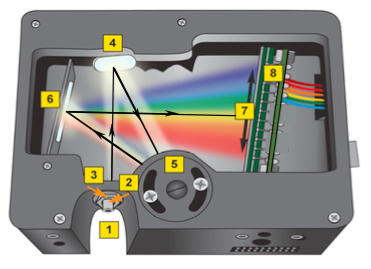
\includegraphics[width=\textwidth]{usb4000.png}
\caption[]{The interior of the USB4000 Spectrograph. Fig. from (Ocean Optics).\footnotemark}
\label{fig: usb4000}
\end{figure}
\footnotetext{\url{http://oceanoptics.com/product/usb4000-custom/}}
}

Light enters the optical bench inside the USB4000 through a light limiting slit (3). If needed the light can be passed through a fiber which connects via the connectors (1-2). A collimating  mirror (4) reflects the light toward the grating. The grating (5) deflects the light on  to a mirror (6) that focus the light on to a lens. The lens (7) focus the light on to the pixels of the CCD detector (8).




















